%%
%% MPLID - GigaScience Data Note
%% Membrane Protein-Lipid Interface Dataset
%% Oxford University Press / GigaScience Template
%%

\documentclass[unnumsec,webpdf,contemporary,large,numbered]{oup-authoring-template}

\graphicspath{{figures/}}

\begin{document}

\journaltitle{GigaScience}
\copyrightyear{2026}
\pubyear{2026}
\appnotes{Data Note}

\firstpage{1}

\title[MPLID: Membrane Protein-Lipid Interface Dataset]{MPLID: A Large-Scale Dataset of Experimentally Validated Membrane Protein-Lipid Contact Residues for Machine Learning}

\author[1,2,$\ast$]{Folorunsho Bright Omage\ORCID{0000-0002-9750-5034}}
\author[1]{Ivan Mazoni}
\author[1]{In\'{a}cio Henrique Yano}
\author[1,$\ast$]{Goran Neshich}

\address[1]{\orgdiv{Computational Biology Research Group}, \orgname{Embrapa Digital Agriculture}, \orgaddress{\street{Av. Andr\'{e} Tosello 209}, \postcode{13083-886}, \state{Campinas, S\~{a}o Paulo}, \country{Brazil}}}
\address[2]{\orgdiv{Biological Chemistry Laboratory, Department of Organic Chemistry, Institute of Chemistry}, \orgname{University of Campinas (UNICAMP)}, \orgaddress{\street{R. Monteiro Lobato 270}, \postcode{13083-970}, \state{Campinas, S\~{a}o Paulo}, \country{Brazil}}}

\corresp[$\ast$]{Corresponding authors. \href{mailto:omagefolorunsho@gmail.com}{omagefolorunsho@gmail.com}; \href{mailto:goran.neshich@embrapa.br}{goran.neshich@embrapa.br}}

\abstract{\textbf{Context:} Membrane proteins constitute approximately 20--30\% of all proteomes and represent over 60\% of current drug targets. Although lipid-protein interactions are essential for membrane protein folding, stability, and function, existing structural datasets predominantly address the question of whether a residue lies within the membrane zone, a property derived from computational hydrophobicity-based positioning algorithms. This conflation obscures a fundamentally different biological question: which residues make direct physical contact with lipid molecules? Answering this question from experimental data is critical for understanding lipid-mediated allostery, designing lipid-mimetic therapeutics, and training accurate machine learning models for lipid binding site prediction.
\textbf{Findings:} We present MPLID (Membrane Protein-Lipid Interface Dataset), a curated residue-level dataset comprising 3,192 non-redundant membrane proteins, 5,134,242 residues, and 38,435 experimentally validated lipid contact annotations (0.75\% positive rate). Labels are derived exclusively from crystallized lipid molecules resolved in Protein Data Bank structures, using a 4.0~\AA{} C$\alpha$-to-lipid-atom distance cutoff that captures van der Waals contacts. The dataset recognizes 121 lipid chemical component codes spanning phospholipids, sphingolipids, sterols, fatty acids, and detergent mimetics. To prevent data leakage, proteins are clustered at 30\% sequence identity using MMseqs2, yielding 594 clusters that are partitioned into training (1,840 proteins), validation (811 proteins), and test (541 proteins) splits. Amino acid composition analysis reveals biologically consistent enrichment of glycine (2.85$\times$), alanine (1.63$\times$), phenylalanine (1.42$\times$), and serine (1.40$\times$) at lipid contact sites, with concomitant depletion of charged residues.
\textbf{Conclusions:} MPLID addresses a distinct biological question compared to existing membrane zone datasets: identifying residues that directly contact lipid molecules rather than those positioned within the membrane hydrophobic slab. With 59 times more proteins and 342 times more residues than the DREAMM benchmark, MPLID enables development of deep learning models for lipid contact prediction, a task with direct applications in structure-guided drug design and membrane protein engineering. The dataset adheres to FAIR principles and is freely available under a CC0 public domain dedication.}

\keywords{membrane proteins, lipid-protein interactions, protein structure, machine learning benchmark, structural biology, experimental validation, residue-level classification, FAIR data}

\maketitle


% ============================================================
\section{Context}
% ============================================================

Membrane proteins are central to virtually all cellular processes, mediating transport of ions and solutes, signal transduction, energy conversion, and cell adhesion \cite{wallin1998}. Genomic analyses consistently estimate that 20--30\% of open reading frames in any given proteome encode membrane proteins \cite{wallin1998}, and pharmacological surveys have established that these proteins account for more than 60\% of all current drug targets \cite{overington2006, santos2017}. Despite their biomedical importance, membrane proteins remain among the most challenging targets for structural and computational biology, in large part because their native functional context, the lipid bilayer, is difficult to recapitulate experimentally and model computationally.

A growing body of evidence demonstrates that lipid-protein interactions are not passive consequences of membrane embedding but rather active modulators of protein structure, dynamics, and function \cite{corradi2019, laganowsky2014}. Specific lipid binding events regulate ion channel gating \cite{duncan2020}, G protein-coupled receptor (GPCR) signaling \cite{bhattacharya2021}, and transporter conformational cycling \cite{lee2004}. Cholesterol, for example, occupies defined binding sites on GPCRs that are structurally resolved at atomic resolution \cite{hanson2008}, and cardiolipin binding is essential for the function of mitochondrial respiratory chain complexes \cite{contreras2012}. The diversity of lipid species in biological membranes, encompassing phospholipids, sphingolipids, sterols, and glycolipids \cite{harayama2018, vanmeer2008}, creates a complex interaction landscape that shapes the behavior of membrane-embedded proteins.

\subsection{Membrane zone versus lipid contact: two distinct questions}

A fundamental distinction exists between two related but different biological questions in membrane protein structural biology. The first question, ``Is this residue located within the membrane zone?'', has been addressed by computational databases such as the Orientations of Proteins in Membranes (OPM) database \cite{lomize2012, lomize2006}. OPM positions membrane proteins in a hydrophobic slab model using energy minimization against experimentally calibrated transfer free energy parameters, producing membrane boundaries for over 15,000 protein entries. This approach is invaluable for understanding membrane protein topology, but the resulting labels reflect a coarse spatial localization: typically 20--40\% of residues in a transmembrane protein fall within the OPM-defined membrane zone.

The second question, ``Does this residue make direct physical contact with a lipid molecule?'', requires experimental structural evidence. Crystallographic and cryo-electron microscopy structures frequently resolve lipid molecules at specific protein surface sites, revealing native lipid interaction partners at atomic resolution. These experimental contacts represent a far more stringent and specific annotation: in our dataset, only 0.75\% of residues in membrane proteins make lipid contacts within 4.0~\AA{}, a rate approximately 30--50 times lower than the membrane zone positive rate.

This distinction has profound consequences for both biological interpretation and machine learning model development (Table~\ref{tab:distinction}). Membrane zone labels identify the general region of a protein that is embedded in the bilayer, while lipid contact labels pinpoint specific binding sites that may mediate functionally important lipid-protein interactions. For drug discovery, the latter is far more actionable: lipid contact sites represent potential targets for allosteric modulation by lipid-mimetic compounds \cite{chatzigoulas2022server}, while membrane zone annotations provide no such site-level resolution.

\begin{table}[tbp]
\centering
\caption{Comparison of membrane zone and lipid contact prediction tasks. These represent fundamentally different biological questions with distinct label sources, positive rates, and downstream applications.}
\label{tab:distinction}
\small
\begin{tabular}{@{}p{2.2cm}p{2.5cm}p{2.5cm}@{}}
\toprule
\textbf{Aspect} & \textbf{Membrane zone} & \textbf{Lipid contact} \\
\midrule
Label source & Computational (OPM) & Experimental (PDB) \\
Biological question & In membrane slab? & Contacts lipid? \\
Positive rate & 20--40\% & $\sim$0.75\% \\
Spatial resolution & Zone-level ($\sim$30~\AA) & Atomic (4.0~\AA) \\
Validation & In silico energy & X-ray/cryo-EM \\
Key application & Topology prediction & Binding site identification \\
\bottomrule
\end{tabular}
\end{table}

\subsection{Existing resources and their limitations}

Several resources provide information about membrane protein-lipid interactions, each with specific scope and limitations. The OPM database \cite{lomize2012} remains the definitive resource for membrane protein positioning, providing computationally derived membrane boundaries for transmembrane and peripheral proteins. However, OPM labels represent theoretical membrane zones rather than experimentally resolved lipid interaction sites.

The MemProtMD database \cite{newport2019, stansfeld2015} complements OPM by providing coarse-grained molecular dynamics simulations of membrane proteins embedded in explicit phospholipid bilayers. While MemProtMD offers valuable insights into lipid organization around proteins, its contacts derive from simulations rather than experimental structures, and the database focuses on integral membrane proteins in a single lipid type (dipalmitoylphosphatidylcholine).

For machine learning applications, the DREAMM dataset \cite{chatzigoulas2022} established an important benchmark with 54 peripheral membrane proteins (later expanded to 65) annotated with experimentally validated membrane-penetrating residues. DREAMM demonstrated that ensemble machine learning can achieve a Matthews correlation coefficient (MCC) of 0.84 for predicting protein-membrane interfaces \cite{chatzigoulas2022}. However, the limited scale of DREAMM (approximately 15,000 residues) constrains the development of deep learning approaches that benefit from larger training sets. More recently, PMIpred introduced a physics-informed transformer approach trained on molecular dynamics data for peptide-membrane interactions \cite{vanhilten2024}, and protein language model approaches have been explored using ProtTrans embeddings \cite{paranou2024, elnaggar2022}.

\subsection{The need for large-scale experimental lipid contact data}

The convergence of three trends motivates the creation of MPLID. First, the rapid growth of the Protein Data Bank \cite{berman2000, burley2023}, which now contains over 220,000 structures, means that thousands of membrane protein structures with resolved lipid molecules are available for systematic analysis. Second, advances in protein language models such as ESM-2 \cite{lin2023} and ProtTrans \cite{elnaggar2022} have demonstrated that per-residue embeddings trained on evolutionary data can capture structural and functional properties, but training supervised models on top of these representations requires large labeled datasets. Third, structure-guided drug discovery increasingly recognizes lipid binding sites as druggable targets for allosteric modulation \cite{chatzigoulas2022server, duncan2020}, creating demand for systematic catalogs of experimentally validated lipid interaction sites.

MPLID addresses these needs by providing experimentally validated lipid contact annotations for 3,192 membrane proteins containing 5,134,242 residues, representing a 59-fold increase in protein count and a 342-fold increase in residue count compared to DREAMM. All labels derive from crystallized lipid molecules in PDB structures, ensuring experimental ground truth at atomic resolution.


% ============================================================
\section{Data Description}
% ============================================================

\subsection{Dataset overview}

MPLID provides residue-level binary annotations indicating whether each residue in a membrane protein makes direct physical contact with a crystallized lipid molecule. The complete dataset encompasses 3,192 membrane proteins with a total of 5,134,242 residues, of which 38,435 (0.75\%) are labeled as lipid contacts (Table~\ref{tab:overview}). This low positive rate reflects the biological reality that only a small fraction of residues in membrane proteins make direct lipid contacts within 4.0~\AA{}, even among proteins that are fully embedded in lipid bilayers. The remaining residues are located in solvent-exposed domains, protein-protein interfaces, or interior regions of multi-subunit complexes.

\begin{table}[tbp]
\centering
\caption{MPLID dataset summary statistics. All labels are derived from crystallized lipid molecules in PDB structures using a 4.0~\AA{} C$\alpha$-to-lipid-atom distance cutoff.}
\label{tab:overview}
\begin{tabular}{@{}lr@{}}
\toprule
\textbf{Metric} & \textbf{Value} \\
\midrule
Total proteins & 3,192 \\
Total residues & 5,134,242 \\
Lipid contact residues & 38,435 \\
Contact rate & 0.75\% \\
Sequence clusters (30\% identity) & 594 \\
Recognized lipid codes & 121 \\
Distance cutoff & 4.0~\AA \\
Label source & Experimental only \\
\bottomrule
\end{tabular}
\end{table}

Proteins in the dataset range from 22 to 9,493 residues (median 1,030; mean 1,609), reflecting the diversity of membrane protein sizes from small single-pass transmembrane peptides to large multi-subunit complexes. The number of lipid contacts per protein ranges from 0 to 418 (median 4; mean 12), with 410 proteins having zero contacts despite containing crystallized lipid molecules in their PDB entries; these cases arise when lipid molecules are resolved in the structure but positioned beyond the 4.0~\AA{} contact threshold from protein residues.

\subsection{Data schema and format}

Each record in MPLID contains ten fields that provide complete information for each annotated residue. The \texttt{pdb\_id} field contains the four-character PDB accession code, and \texttt{chain\_id} specifies the polypeptide chain within the structure. The \texttt{residue\_number} gives the residue's position in the chain, while \texttt{residue\_name} provides the three-letter amino acid code. The binary label \texttt{is\_contact} takes a value of 1 for residues whose C$\alpha$ atom is within 4.0~\AA{} of any lipid heavy atom and 0 otherwise. The \texttt{label\_source} field is set to ``EXPERIMENTAL'' for all entries, confirming that labels derive from crystallized lipids rather than computational predictions. The \texttt{confidence} field provides a quality metric, and \texttt{min\_distance} records the minimum distance in Angstroms between the residue and the nearest lipid molecule. Finally, \texttt{cluster\_id} assigns each protein to a sequence cluster, and \texttt{split} indicates assignment to training, validation, or test partitions.

Data are distributed as gzip-compressed CSV files partitioned by split (train, validation, test), along with a protein-level metadata file containing per-protein summary statistics including residue counts, contact counts, contact rates, cluster assignments, and split assignments.

\subsection{Train/validation/test splits}

The dataset is partitioned into training (1,840 proteins; 2,634,209 residues), validation (811 proteins; 1,632,603 residues), and test (541 proteins; 867,430 residues) splits (Table~\ref{tab:splits}; Figure~\ref{fig:overview}). Critically, splitting is performed at the protein level with cluster-aware stratification: proteins within the same sequence cluster are always assigned to the same split, preventing data leakage from sequence-similar proteins appearing in both training and evaluation partitions. This design choice is essential for meaningful generalization assessment, as protein-level leakage can dramatically inflate performance estimates in structural bioinformatics tasks.

\begin{table}[tbp]
\centering
\caption{Train/validation/test split statistics. Proteins within the same sequence cluster (30\% identity) are always assigned to the same split. Contact rates vary slightly across splits due to cluster-level stratification.}
\label{tab:splits}
\begin{tabular}{@{}lrrr@{}}
\toprule
\textbf{Split} & \textbf{Proteins} & \textbf{Residues} & \textbf{Rate (\%)} \\
\midrule
Training & 1,840 & 2,634,209 & 0.85 \\
Validation & 811 & 1,632,603 & 0.60 \\
Test & 541 & 867,430 & 0.70 \\
\midrule
Total & 3,192 & 5,134,242 & 0.75 \\
\bottomrule
\end{tabular}
\end{table}

\begin{figure*}[tbp]
\centering
\includegraphics[width=\textwidth]{fig1_dataset_overview.pdf}
\caption{MPLID dataset overview. (A) Distribution of proteins across training (57.6\%), validation (25.4\%), and test (16.9\%) splits. (B) Class distribution showing the severe imbalance between contact (0.75\%) and non-contact (99.25\%) residues. (C) Total residues per split. (D) Contact rates across splits, showing slight variation due to cluster-level stratification. All splits maintain the same approximate class imbalance.}
\label{fig:overview}
\end{figure*}

The cluster-aware splitting strategy uses MMseqs2 \cite{steinegger2017} with a 30\% sequence identity threshold and 80\% alignment coverage, producing 594 clusters. Entire clusters are assigned to splits to ensure that no protein in the validation or test sets shares more than 30\% sequence identity with any training protein. This threshold is substantially more conservative than the 40\% identity commonly used in protein function prediction benchmarks \cite{sillitoe2021}, further reducing the risk of overestimating generalization performance.

\subsection{Sequence clustering analysis}

The 594 sequence clusters exhibit a highly skewed size distribution. The largest cluster contains 95 proteins, while 259 clusters (43.6\%) contain only a single protein, reflecting the sequence diversity of membrane proteins across different families and superfamilies. This clustering pattern indicates substantial structural and functional diversity in the dataset, as singleton clusters represent unique membrane protein families without close homologs.


% ============================================================
\section{Data Validation}
% ============================================================

\subsection{Amino acid composition at lipid contact sites}

Analysis of amino acid enrichment at lipid contact sites reveals biologically meaningful and interpretable patterns (Figure~\ref{fig:enrichment}). Enrichment ratios were calculated as the fraction of each amino acid among contact residues divided by its fraction in the complete dataset. Glycine exhibits the strongest enrichment (2.85$\times$), consistent with its minimal side chain that permits close approach of lipid acyl chains to the protein backbone and its prevalence at helix-helix interfaces in transmembrane domains where lipid molecules can intercalate. Alanine (1.63$\times$) is similarly enriched, reflecting both its hydrophobic character and its prevalence in transmembrane helices. Among aromatic residues, phenylalanine (1.42$\times$) and tryptophan (1.31$\times$) show clear enrichment, in agreement with the well-documented preference of aromatic residues for the membrane-water interface region where they can interact with lipid headgroups through cation-$\pi$ and hydrogen bonding interactions \cite{corradi2019}. Serine, despite being polar, shows notable enrichment (1.40$\times$), likely reflecting its role in hydrogen bonding with lipid headgroups at the membrane interface.

\begin{figure}[tbp]
\centering
\includegraphics[width=\columnwidth]{fig2_amino_acid_enrichment.pdf}
\caption{Amino acid enrichment at lipid contact sites. Enrichment ratios are calculated as the frequency of each amino acid among contact residues divided by its overall frequency in the dataset. Colors indicate amino acid physicochemical properties: hydrophobic (orange), polar (blue), positive charge (red), negative charge (purple), and special (gray). The dashed line marks the expected frequency (1.0). Values above 1.0 indicate enrichment; values below 1.0 indicate depletion.}
\label{fig:enrichment}
\end{figure}

Conversely, negatively charged residues are strongly depleted at lipid contact sites: glutamic acid (0.32$\times$) and aspartic acid (0.37$\times$) are the most underrepresented amino acids. Positively charged residues are also depleted, with lysine at 0.48$\times$ and arginine at 0.65$\times$, although the depletion is less severe than for negatively charged residues. This pattern is consistent with the energetic penalty of burying charged groups in the hydrophobic membrane interior. Interestingly, histidine (0.97$\times$) is nearly neutral, which may reflect its ability to adopt both charged and uncharged states depending on the local pH environment near the membrane surface.

Among the branched-chain hydrophobic residues, leucine (0.63$\times$), isoleucine (0.64$\times$), and valine (0.53$\times$) are depleted despite their hydrophobic character. This reflects the distinction between membrane embedding and lipid contact: these residues are highly abundant in the tightly packed hydrophobic core of transmembrane helix bundles, where interhelical packing excludes lipid molecules. Crystallized lipids are predominantly resolved at protein surface sites, interfacial regions, and specific binding pockets rather than within the helix bundle interior, explaining why residues enriched in the transmembrane core are underrepresented among lipid contacts.

\subsection{Distance distribution analysis}

The distribution of minimum distances between protein residues and lipid molecules provides independent validation of the 4.0~\AA{} contact cutoff (Figure~\ref{fig:distance}). Among contact residues, the distance distribution shows a clear peak at approximately 3.5--4.0~\AA{}, corresponding to typical van der Waals contact distances between heavy atoms. The sharp boundary at 4.0~\AA{} indicates that the cutoff effectively captures the transition from direct physical contact to non-contact. For non-contact residues, the distribution is broadly shifted toward larger distances, with a peak near 8--12~\AA{} and a long tail extending to distances greater than 30~\AA{} for residues in soluble domains far from any lipid molecule.

\begin{figure}[tbp]
\centering
\includegraphics[width=\columnwidth]{fig3_distance_distribution.pdf}
\caption{Distribution of minimum residue-to-lipid distances. (A) Contact residues ($\leq$4.0~\AA) show a peak near 3.5--4.0~\AA{}, consistent with van der Waals contact distances. (B) Non-contact residues display a broad distribution with distances extending well beyond 30~\AA{}, confirming clear separation between contacting and non-contacting populations.}
\label{fig:distance}
\end{figure}

\subsection{Protein size and contact density distributions}

The distribution of protein sizes in MPLID spans three orders of magnitude, from small peptides (22 residues) to large multi-subunit complexes (9,493 residues). The median size of 1,030 residues and the interquartile range of 472--1,953 residues reflect the predominance of multi-pass transmembrane proteins (Figure~\ref{fig:proteinstats}). Contact density, defined as the fraction of residues making lipid contacts, varies substantially across proteins. The median contact rate of 0.46\% and mean of 0.96\% confirm the extreme class imbalance inherent to this prediction task.

\begin{figure}[tbp]
\centering
\includegraphics[width=\columnwidth]{fig4_protein_statistics.pdf}
\caption{Protein-level statistics. Distribution of protein sizes and contact densities across the MPLID dataset, illustrating the diversity of membrane protein families represented.}
\label{fig:proteinstats}
\end{figure}

\subsection{Comparison with existing resources}

MPLID provides a substantial increase in scale compared to existing experimentally validated membrane protein-lipid contact datasets (Figure~\ref{fig:dreamm}; Table~\ref{tab:comparison}). The DREAMM dataset \cite{chatzigoulas2022}, the most rigorous prior benchmark for membrane protein-lipid interface prediction, contains 54 proteins with approximately 15,000 residues. MPLID expands this by a factor of 59 in protein count and 342 in residue count, while maintaining the same commitment to experimental ground truth from resolved crystal structures. An important difference in scope should be noted: DREAMM focuses exclusively on peripheral membrane proteins that associate with a single leaflet, while MPLID encompasses all membrane protein classes, including integral multi-pass transmembrane proteins, single-pass proteins, and peripheral proteins. This broader scope means that MPLID and DREAMM are complementary rather than directly substitutable benchmarks, and models trained on one may not transfer directly to the other without domain adaptation. The increased scale of MPLID is particularly important for deep learning approaches, which benefit from larger and more diverse training sets. The diversity of membrane protein families represented in MPLID, spanning 594 sequence clusters at 30\% identity, ensures broad coverage of the membrane protein structural landscape.

\begin{figure}[tbp]
\centering
\includegraphics[width=\columnwidth]{fig5_comparison_dreamm.pdf}
\caption{Scale comparison between MPLID and the DREAMM benchmark dataset \cite{chatzigoulas2022}. (A) Number of proteins (3,192 versus 54; 59$\times$ increase). (B) Number of annotated residues (5,134,242 versus $\sim$15,000; 342$\times$ increase). Both datasets use experimental lipid contact labels from PDB structures.}
\label{fig:dreamm}
\end{figure}

\begin{table*}[tbp]
\centering
\caption{Comparison of MPLID with existing membrane protein-lipid interaction resources. MPLID is the largest dataset providing experimentally validated residue-level lipid contact labels.}
\label{tab:comparison}
\small
\begin{tabular}{@{}lrrll@{}}
\toprule
\textbf{Resource} & \textbf{Proteins} & \textbf{Residues} & \textbf{Label type} & \textbf{Label source} \\
\midrule
MPLID (this work) & 3,192 & 5,134,242 & Lipid contact & Experimental (PDB) \\
DREAMM \cite{chatzigoulas2022} & 54 & $\sim$15,000 & Membrane interface & Experimental (PDB) \\
OPM \cite{lomize2012} & 15,096 & -- & Membrane zone & Computational \\
MemProtMD \cite{newport2019} & $\sim$5,400 & -- & Lipid contact & Simulated (CG-MD) \\
\bottomrule
\end{tabular}
\end{table*}

It is important to note that MPLID and OPM address different biological questions and should be viewed as complementary rather than competing resources. OPM provides membrane zone annotations that are useful for topology prediction and membrane protein classification, while MPLID provides lipid contact annotations that are useful for binding site identification and lipid-mediated function analysis. Models trained on one type of label cannot be directly evaluated on the other, and researchers should select the appropriate dataset based on their specific biological question.

\subsection{Lipid type diversity}

MPLID recognizes 121 lipid chemical component codes from the PDB Chemical Component Dictionary, organized into six functional categories. Phospholipids include cardiolipin (CDL, found in 675 structures), phosphocholine variants (PCW, 196 structures), phosphoethanolamine (PEE, 273 structures), and phosphoglycerol (PGV, 144 structures). Sterols are represented by cholesterol (CLR, 1,119 structures) and derivatives including cholesterol hemisuccinate (CHD, 151 structures) and cholesteryl oleate (Y01, 483 structures). Fatty acids include palmitate (PLM, 734 structures), oleic acid (OLA, 379 structures), myristate (MYR, 426 structures), and stearate (STE, 94 structures). Sphingolipids include sphingosine (SPH, 102 structures) and sphingosine-1-phosphate (S1P, 16 structures). Detergent mimetics used in crystallization, which often occupy native lipid binding sites, include lauryl maltose neopentyl glycol (LMT, 677 structures), n-dodecyl-$\beta$-D-maltoside (BOG, 510 structures), and lauryldimethylamine oxide (LDA, 263 structures). This comprehensive lipid recognition ensures that MPLID captures the full diversity of protein-lipid interactions observed in experimental structures.

\subsection{Structural visualization of lipid contacts}

To illustrate the nature of the lipid contact annotations in MPLID, representative membrane protein structures with their resolved lipid molecules are shown in Figure~\ref{fig:structures}. These examples demonstrate that lipid contacts occur at specific, well-defined sites on the protein surface rather than uniformly across the membrane-exposed region. Contact residues (highlighted in red/orange) are interspersed with non-contact residues even in transmembrane regions, confirming that lipid contact prediction is a more specific task than membrane zone classification.

\begin{figure*}[tbp]
\centering
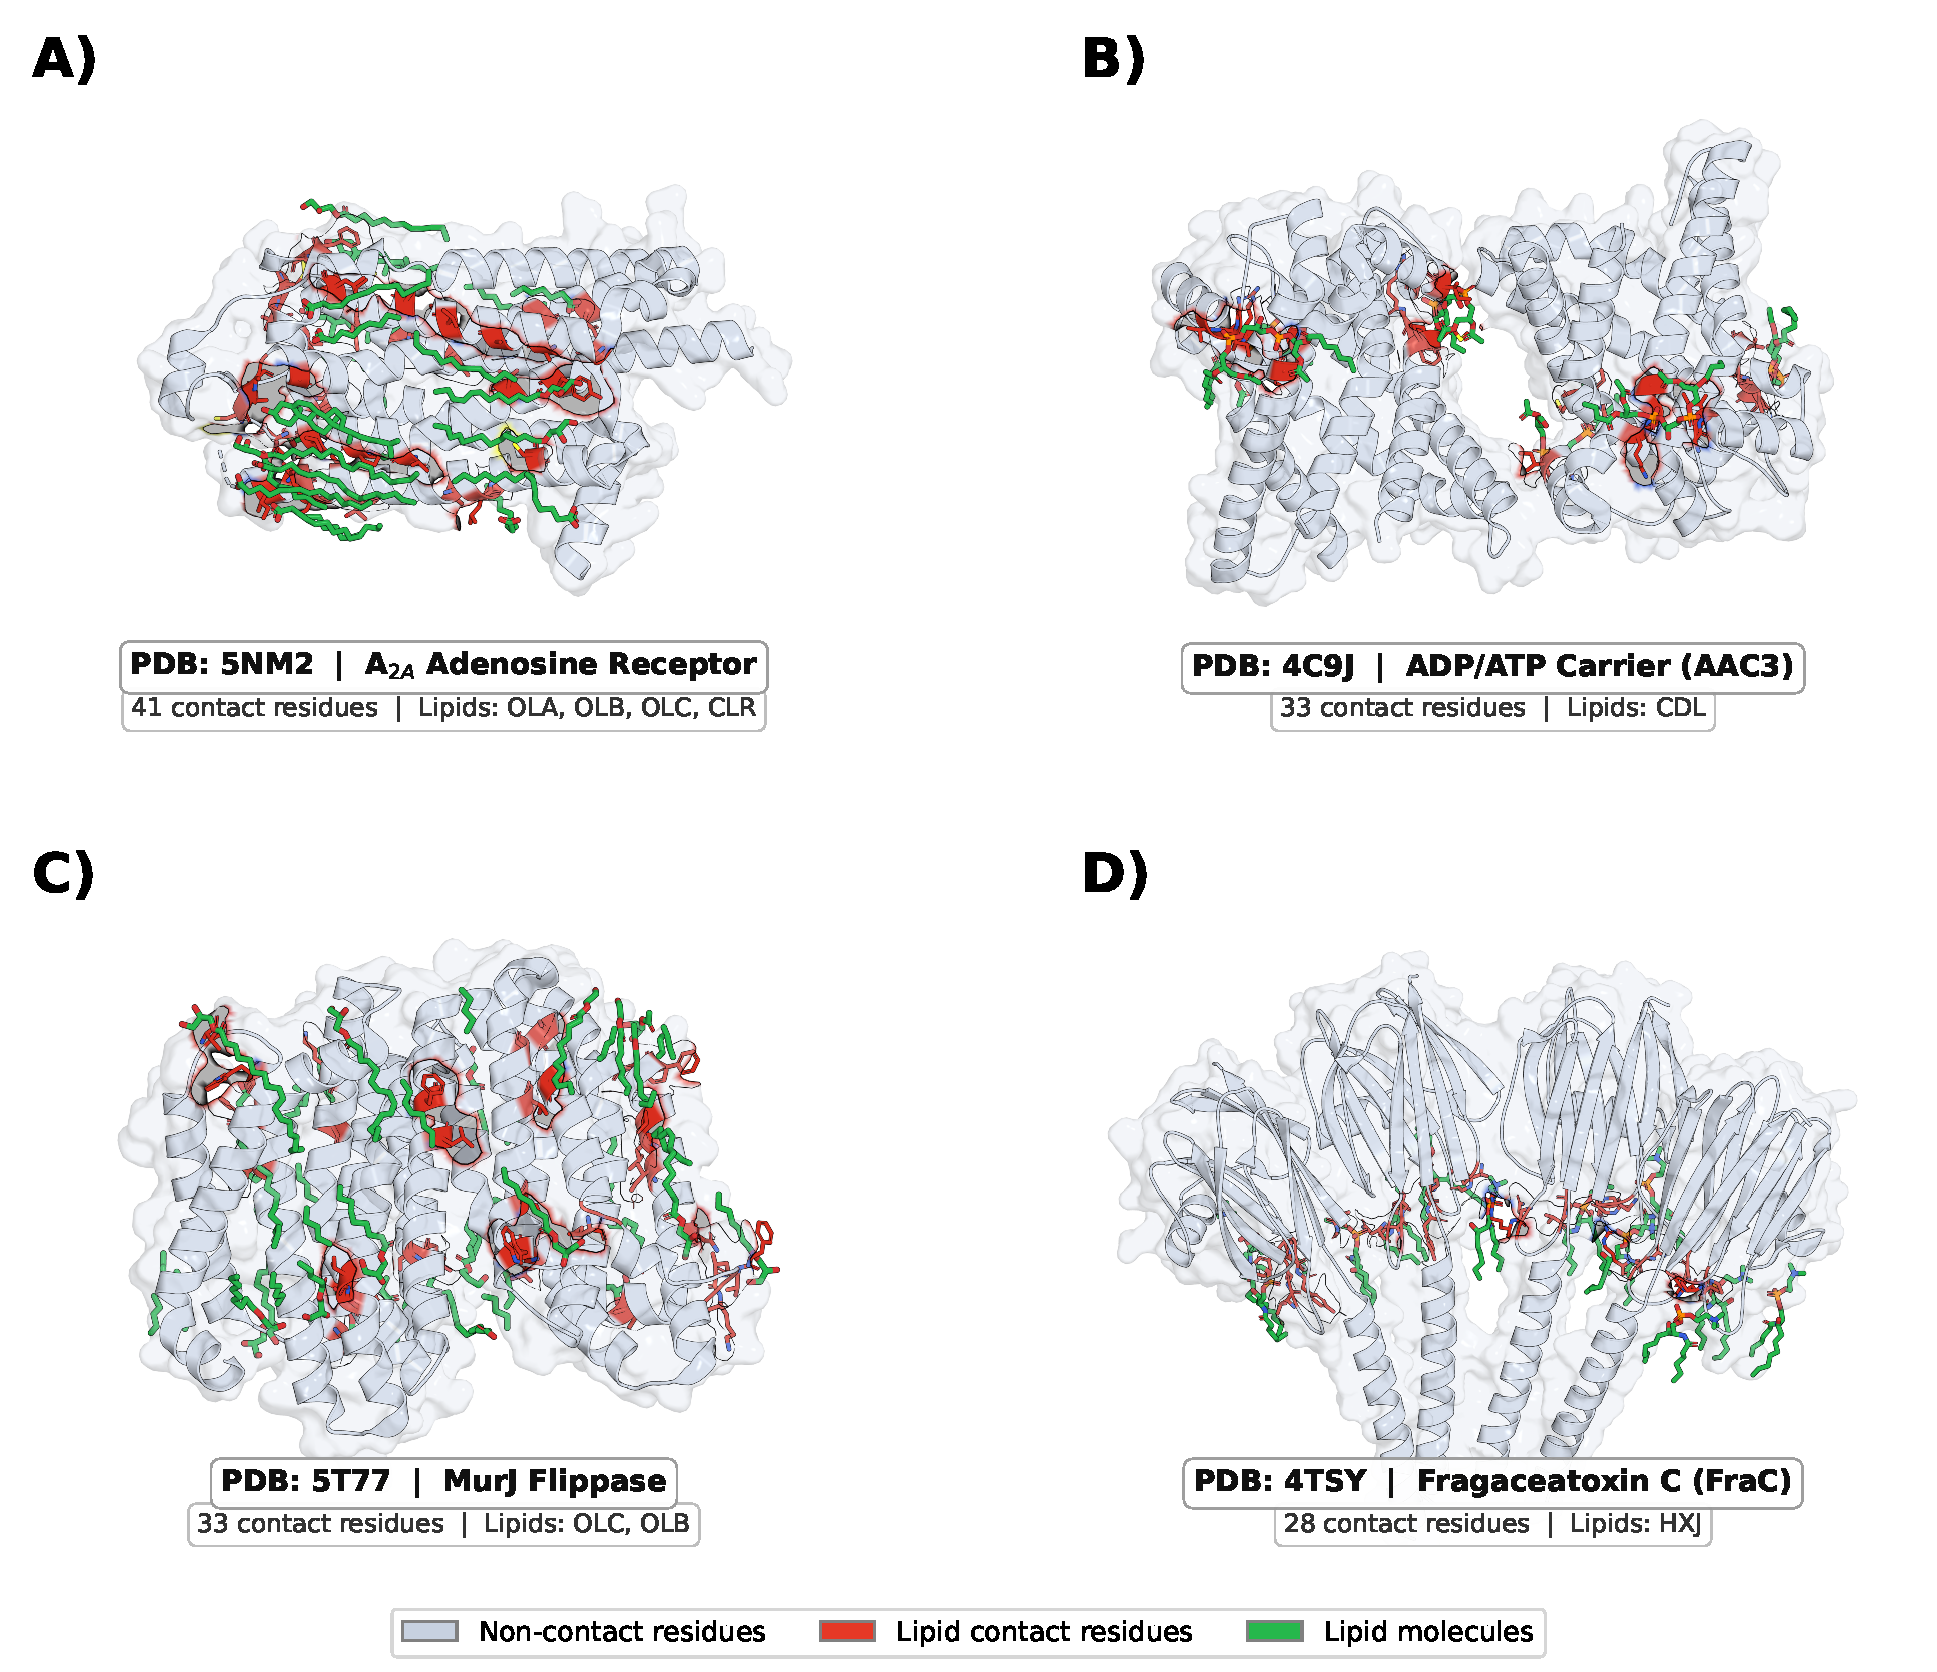
\includegraphics[width=\textwidth]{fig7_structural_visualization.pdf}
\caption{Structural visualization of MPLID lipid contact annotations across four representative membrane protein classes, rendered with PyMOL. Protein backbone is shown in gray cartoon, lipid-contacting residues are highlighted in coral/red with side-chain sticks, and crystallized lipid molecules are displayed as green sticks. A semi-transparent molecular surface provides spatial context. (A) A\textsubscript{2A} adenosine receptor (PDB: 5NM2), a GPCR with 41 contact residues and four lipid types (oleic acid, cholesterol). (B) ADP/ATP carrier AAC3 (PDB: 4C9J), a mitochondrial transporter with 33 cardiolipin contact residues across two chains. (C) MurJ flippase (PDB: 5T77), a lipid II flippase with 33 contacts distributed across its transmembrane helices. (D) Fragaceatoxin C (PDB: 4TSY), a tetrameric pore-forming toxin with 28 sphingolipid contacts at the membrane insertion interface. These examples demonstrate that lipid contacts are site-specific rather than uniformly distributed across membrane-exposed surfaces.}
\label{fig:structures}
\end{figure*}


% ============================================================
\section{Methods}
% ============================================================

\subsection{Data source integration}

MPLID was constructed by integrating two primary data sources to identify membrane proteins with experimentally resolved lipid contacts. From the Orientations of Proteins in Membranes (OPM) database \cite{lomize2012}, we obtained a list of 15,096 validated membrane proteins, ensuring that only bona fide membrane proteins were included in the dataset. The OPM database was used exclusively for protein identification and classification; OPM-derived membrane zone labels were not used for residue annotation. From the RCSB Protein Data Bank \cite{berman2000, burley2023}, we queried all structures containing recognized lipid chemical components, identifying 8,221 structures with lipid ligands. The intersection of these two sets, 3,329 candidate membrane proteins with potential lipid contacts, formed the input for the processing pipeline (Figure~\ref{fig:cluster}).

\begin{figure}[tbp]
\centering
\includegraphics[width=\columnwidth]{fig6_cluster_analysis.pdf}
\caption{Sequence cluster analysis. Distribution of cluster sizes at 30\% sequence identity, showing that the majority of clusters are singletons while a small number contain many homologous structures. The inset shows the pipeline filtering from OPM/RCSB intersection to the final processed dataset.}
\label{fig:cluster}
\end{figure}

\subsection{Lipid molecule identification}

Lipid molecules in PDB structures were identified using their Chemical Component Dictionary codes. We compiled a list of 121 lipid codes organized into six functional categories: phospholipids (CDL, POV, PCW, PEE, PGV, PLM, and others), sphingolipids (SPH, S1P, HXJ), sterols (CLR, CHD, Y01, BCL), fatty acids (MYR, OLA, STE, ARA, DHA), detergent mimetics (LDA, LMT, BOG, OLC, DPC), and other membrane-associated molecules (EPE, UNL). This list was developed iteratively by cross-referencing the PDB Chemical Component Dictionary with lipid classification databases and manually curating entries to exclude non-lipid small molecules that might share similar chemical codes. Detergent mimetics were included because they frequently occupy native lipid binding sites in membrane protein crystal structures and provide relevant information about lipid-protein interaction geometry \cite{lee2004}.

\subsection{Structure processing and contact calculation}

For each candidate protein, the original PDB coordinate file was downloaded from RCSB to preserve HETATM records containing lipid molecule coordinates. Structure parsing was performed using BioPython \cite{cock2009}, extracting all standard amino acid residues (ATOM records) and all recognized lipid molecules (HETATM records). Non-standard residues, water molecules, metal ions, and non-lipid ligands were excluded.

Lipid contacts were defined using a distance-based criterion. For each protein residue $R$, represented by its C$\alpha$ atom, and each lipid molecule $L$ in the structure, the minimum distance $d_{\min}(R, L)$ between the C$\alpha$ atom of $R$ and any heavy (non-hydrogen) atom of $L$ was calculated. A residue was labeled as a lipid contact if:

\begin{equation}
d_{\min}(R, L) = \min_{b \in L} \| \mathbf{r}_{\text{C}\alpha}^{R} - \mathbf{r}_b \| \leq 4.0~\text{\AA}
\label{eq:contact}
\end{equation}

\noindent where $\mathbf{r}_{\text{C}\alpha}^{R}$ denotes the Cartesian coordinates of the C$\alpha$ atom of residue $R$ and $\mathbf{r}_b$ denotes the coordinates of heavy atom $b$ in lipid $L$. The use of C$\alpha$ atoms as residue representatives provides a consistent and unambiguous reference point across all amino acid types, avoiding the variability introduced by differing side chain conformations and missing atoms in crystal structures. The 4.0~\AA{} cutoff was chosen to capture van der Waals contacts at C$\alpha$ resolution, consistent with standard distance thresholds in protein-ligand interaction analysis. For each residue, the minimum C$\alpha$-to-lipid distance was recorded regardless of contact status, providing a continuous distance metric that enables researchers to evaluate alternative cutoff values.

\subsection{Quality filtering}

Of the 3,329 candidate proteins, 3,202 (96.2\%) were successfully processed, with failures arising from corrupted PDB files, non-standard chain identifiers, or structures lacking parseable protein residues. An additional 10 proteins were excluded during quality filtering because they contained no standard amino acid residues with resolved C$\alpha$ atoms, yielding 3,192 proteins with valid residue-level annotations. Among these, 2,792 (87.4\%) contained at least one residue within 4.0~\AA{} of a lipid molecule. The final dataset includes all 3,192 proteins (including those with zero contacts), as negative examples from lipid-free proteins provide valuable training signal by establishing that not all membrane protein residues contact lipids.

\subsection{Sequence clustering}

To prevent data leakage between training, validation, and test splits, all 3,192 proteins were clustered using MMseqs2 \cite{steinegger2017} with a 30\% sequence identity threshold and 80\% bidirectional alignment coverage. These stringent thresholds ensure that proteins assigned to different splits are sufficiently divergent in sequence to represent independent test cases. The clustering produced 594 clusters, with the largest cluster containing 95 members and 259 clusters containing a single protein.

\subsection{Split strategy}

Clusters were assigned to training, validation, and test splits using stratified random sampling at the cluster level, with stratification based on the average contact rate per cluster. This approach ensures that each split contains a representative distribution of high-contact and low-contact proteins. Entire clusters were assigned to a single split, guaranteeing that no two proteins sharing more than 30\% sequence identity appear in different partitions. The resulting splits contain 1,840 training proteins (57.6\%), 811 validation proteins (25.4\%), and 541 test proteins (16.9\%).

\subsection{Software and computational environment}

The MPLID construction pipeline was implemented in Python 3.11.8 using BioPython 1.83 \cite{cock2009} for PDB structure parsing, pandas 2.2.2 \cite{mckinney2010} for data manipulation, NumPy 1.26.4 for numerical computation, SciPy 1.13 for distance calculations, and scikit-learn 1.7.2 \cite{pedregosa2011} for data splitting. MMseqs2 version 15 \cite{steinegger2017} was used for sequence clustering. The RCSB PDB search API was used for programmatic identification of structures containing lipid chemical components.


% ============================================================
\section{Re-use Potential}
% ============================================================

MPLID is designed to serve as a general-purpose benchmark and training resource for multiple research applications in structural bioinformatics, drug discovery, and membrane biology.

\subsection{Machine learning benchmark for lipid contact prediction}

The primary intended use of MPLID is as a benchmark dataset for developing and evaluating machine learning models that predict lipid contact residues from protein sequence or structure. The pre-defined, cluster-aware train/validation/test splits enable standardized model comparison, and the severe class imbalance (0.75\% positive rate) presents a realistic and challenging binary classification task that requires specialized approaches such as class weighting, oversampling \cite{chawla2002}, or focal loss functions. The scale of the dataset is sufficient for training deep neural networks, including architectures that combine structural descriptors with protein language model embeddings from ESM-2 \cite{lin2023} or ProtTrans \cite{elnaggar2022}. We note that the Matthews correlation coefficient should be used as the primary evaluation metric for this task due to the extreme class imbalance, as accuracy and even F1 scores can be misleading when the negative class dominates.

\subsection{Drug discovery applications}

Lipid binding sites on membrane proteins represent an emerging class of druggable targets. General anesthetics, neurosteroids, and endocannabinoids modulate ion channels and GPCRs through specific lipid binding sites \cite{duncan2020, brannigan2008}, and cholesterol binding sites on GPCRs are increasingly recognized as allosteric modulatory sites \cite{hanson2008, fantini2013}. MPLID can inform the identification of lipid-mimetic drug binding sites by providing a catalog of experimentally validated lipid interaction residues across thousands of membrane proteins. Predicted lipid contact sites on therapeutically relevant proteins can guide the design of lipid-conjugated prodrugs, membrane-anchored therapeutics, or allosteric modulators that exploit lipid binding pockets.

\subsection{Structural biology and protein engineering}

Understanding which residues contact lipids is essential for rational membrane protein engineering. Mutations at lipid contact sites can destabilize membrane proteins, alter their trafficking, or modify their functional properties. MPLID provides data to train models that predict which residues are critical for lipid-mediated stability, enabling more informed design of stabilizing mutations for membrane protein crystallization, cryo-EM, or functional studies. Additionally, the dataset supports comparative analysis of lipid contact patterns across protein families, enabling identification of conserved lipid binding motifs and family-specific interaction signatures.

\subsection{Computational label comparison studies}

The availability of MPLID alongside OPM membrane zone annotations enables systematic comparison of experimental lipid contacts with computational membrane boundaries. To illustrate this capability, we compared MPLID contact labels with OPM-derived membrane zone assignments for the A\textsubscript{2A} adenosine receptor (PDB: 5NM2; Figure~\ref{fig:opm_comparison}). Of the 41 MPLID contact residues, 31 (75.6\%) also fell within the OPM membrane zone (agreement), while 10 residues (24.4\%) were contacted by lipids but located outside the OPM-defined membrane boundaries, likely reflecting interfacial or re-entrant contacts. Conversely, 137 residues were classified as membrane-embedded by OPM but showed no direct lipid contact within 4.0~\AA{}, highlighting the fundamental difference between membrane zone classification and lipid contact prediction. Such studies can quantify the degree to which membrane zone predictions capture actual lipid interaction sites, identify regions where the two annotations diverge (such as re-entrant loops or interfacial amphipathic helices), and inform the development of hybrid annotation schemes that combine both types of information. Researchers working with MemProtMD \cite{newport2019} simulations can similarly compare simulated lipid contacts with the experimental contacts provided by MPLID.

\begin{figure*}[tbp]
\centering
\includegraphics[width=\textwidth]{fig8_opm_comparison.pdf}
\caption{Comparison of MPLID experimental lipid contacts and OPM computational membrane zone for the A\textsubscript{2A} adenosine receptor (PDB: 5NM2). (A) MPLID annotations: lipid-contacting residues (coral/red) with crystallized lipid molecules (green sticks), showing site-specific contacts. (B) OPM membrane zone: residues within the computationally derived membrane boundaries (blue) with the membrane plane markers (spheres). (C) Agreement overlay: residues where both methods agree (green, $n = 31$), MPLID contacts outside the OPM zone (red, $n = 10$), and OPM zone residues without lipid contact (light blue, $n = 137$). This comparison demonstrates that lipid contact prediction is a more specific task than membrane zone classification.}
\label{fig:opm_comparison}
\end{figure*}

\subsection{Integration with protein language models}

The residue-level format of MPLID is directly compatible with per-residue embeddings from protein language models. Each residue's 1,280-dimensional ESM-2 embedding \cite{lin2023} or 1,024-dimensional ProtTrans embedding \cite{elnaggar2022} can be concatenated with structural descriptors and used as input to supervised classifiers. The 594 sequence clusters provide sufficient diversity to evaluate whether language model representations generalize across membrane protein families with limited sequence similarity.


% ============================================================
\section{Availability of Supporting Source Code and Data}
% ============================================================

The complete MPLID dataset is deposited at Zenodo under a CC0 public domain dedication with persistent DOI: [DOI to be assigned upon deposit]. Upon acceptance, the dataset will also be deposited in GigaDB in accordance with journal policy. The Zenodo archive contains the full residue-level annotations (train, validation, and test splits as gzip-compressed CSV files), protein-level metadata, amino acid composition statistics, and a data dictionary describing all fields.

All code for reproducing the dataset from raw PDB structures is available in a public GitHub repository: \url{https://github.com/omagebright/MPLID}. The repository includes the complete processing pipeline (structure downloading, lipid identification, contact calculation, quality filtering, and split generation), analysis scripts for generating figures and tables, and documentation of the data schema and methodology.

The dataset and code are organized following FAIR principles \cite{wilkinson2016}: data are Findable via persistent DOIs and indexed metadata; Accessible through standard HTTPS download from Zenodo and GitHub; Interoperable using standard CSV format with documented column definitions; and Reusable under permissive open licenses (CC0 for data, MIT for code).


% ============================================================
\section{Conflicts of interest}
% ============================================================

The authors declare that they have no competing interests.


% ============================================================
\section{Funding}
% ============================================================

This research was funded by the S\~{a}o Paulo Research Foundation (FAPESP) (grant nos. 2023/02691-2, 2025/23708-6).


% ============================================================
\section{Data availability}
% ============================================================

The data underlying this article are available in Zenodo [DOI to be assigned upon deposit], and in a public GitHub repository at \url{https://github.com/omagebright/MPLID}.


% ============================================================
\section{Author contributions statement}
% ============================================================

Author contributions follow the CRediT taxonomy. F.B.O.: Conceptualization, Methodology, Software, Formal Analysis, Data Curation, Writing (Original Draft), Visualization. I.M.: Validation, Investigation. I.H.Y.: Data Curation, Resources. G.N.: Conceptualization, Supervision, Writing (Review \& Editing), Funding Acquisition. All authors read and approved the final manuscript.


% ============================================================
\section{Ethics approval and consent to participate}
% ============================================================

Not applicable. This study uses publicly available structural data from the Protein Data Bank and does not involve human subjects, animal experiments, or clinical data.


% ============================================================
\section{Consent for publication}
% ============================================================

Not applicable.


% ============================================================
\section{Acknowledgments}
% ============================================================

The authors thank Embrapa Digital Agriculture (Embrapa Agricultura Digital) for computational resources and infrastructure support. The authors acknowledge the RCSB Protein Data Bank \cite{berman2000, burley2023} and the OPM database \cite{lomize2012} teams for maintaining the essential structural biology resources upon which this work depends. The authors thank the developers of MMseqs2 \cite{steinegger2017}, BioPython \cite{cock2009}, and the broader open-source scientific computing community for the software tools used in this study.


% ============================================================
\section{Use of AI-assisted technologies}
% ============================================================

AI-assisted tools (Claude, Anthropic) were used for code development assistance, manuscript drafting, and reference formatting during the preparation of this work. All AI-generated content was critically reviewed, verified, and edited by the authors. The scientific design, data analysis, interpretation, and final manuscript approval were performed entirely by the human authors.


% ============================================================
\section{Abbreviations}
% ============================================================

\noindent
\textbf{MPLID}: Membrane Protein-Lipid Interface Dataset;
\textbf{PDB}: Protein Data Bank;
\textbf{OPM}: Orientations of Proteins in Membranes;
\textbf{GPCR}: G protein-coupled receptor;
\textbf{MCC}: Matthews correlation coefficient;
\textbf{CG-MD}: Coarse-grained molecular dynamics;
\textbf{FAIR}: Findable, Accessible, Interoperable, Reusable;
\textbf{CDL}: Cardiolipin;
\textbf{CLR}: Cholesterol;
\textbf{PLM}: Palmitic acid;
\textbf{DREAMM}: Detection of Residues on Exposed Areas of Membrane-associated Macromolecules;
\textbf{ESM-2}: Evolutionary Scale Modeling 2;
\textbf{SMOTE}: Synthetic Minority Over-sampling Technique;
\textbf{RCSB}: Research Collaboratory for Structural Bioinformatics;
\textbf{CSV}: Comma-separated values.


% ============================================================
% References
% ============================================================

\bibliographystyle{oup-plain}
\bibliography{references}

\end{document}
